\documentclass[acmtog, nonacm]{acmart}

\begin{document}

\title{State of the ART: The Adaptive Radix Tree Index for Main-Memory Databases}

\author{Jonas Fritsch}
\affiliation{
    \institution{Technische Universtität München}
    \department{Fakultät für Informatik}}
\email{fritsch@in.tum.de}

\begin{abstract}
    With recent trends in hardware, main memory capacities have grown to an extent where most traditional DBMS 
    can fit entirely into memory. This change introduced a new shift of the performance bottleneck 
    from disk-based I/O to main memory access.
    
    While previous index structures like the B-Tree were optimized for minimizing disk access, the 
    adaptive radix tree (ART) is a trie-based index structure designed explicitly for in-memory usage. 
    It utilizes newer architecture features like SIMD and caching effectively and compresses its structure 
    dynamically, both horizontal and vertical. With these measures, ART achieves a performance that beats 
    other state-of-the-art order-preserving indexes while having a lower memory footprint at the same time.
\end{abstract}

\maketitle

\section{Introduction}

The architecture of DBMS has constantly been evolving due to advances in hardware. 
Over the last few decades, main memory capacities increased from several megabytes up to thousands 
of gigabytes, such that nowadays, databases can fit entirely into main memory. This change significantly 
impacted the general architecture of DBMS, which resulted in performance improvements 
by several factors \cite{10.1145/1376616.1376713}, \cite{7097722}.

The design of index structures used to query a set of data more efficiently was heavily influenced 
by the main performance bottleneck of disk I/O in traditional disk-based DBMS. 
Original indexes like the B-Tree designed to minimize disk accesses perform poorly 
in an in-memory environment. 
The T-Tree \cite{lehman1985study} was one of the first index structures proposed for main memory DBMS. 
However, over the last 35 years, the hardware landscape changed dramatically, causing T-Trees 
and all other index structures not explicitly designed with caching effects in mind to be rendered 
inefficient for in-memory usage\cite{rao1998cache}. Further focus on developing cache-sensitive index structures resulted in many 
different search tree variants.

Cache-sensitive search trees (CSS-Trees) \cite{rao1998cache}, while utilizing cache lines efficiently, 
introduce a significant overhead for updates as the tree is compactly stored in an array. 
Similarly, the more recent k-ary search tree \cite{10.1145/1565694.1565705} and the Fast Architecture 
Sensitive Tree (FAST) \cite{10.1145/1807167.1807206} both utilize Single Instruction Multiple Data (SIMD) 
instructions for data-level parallelism (DLP) to increase performance. However, as static data 
structures, they do not support incremental updates. A way to circumvent this limitation is to 
use a delta mechanism where another data structure stores differences and is periodically merged 
into the static structure. However, this comes at an additional performance cost. The cache-conscious 
B\textsuperscript{+}-Tree (CSB\textsuperscript{+}) \cite{10.1145/342009.335449} introduced as a variant of 
B\textsuperscript{+}-Trees improves cache utilization by reducing the need to store all different 
child pointers in each node.

Hash-Tables have been a popular indexing choice for main memory databases as they provide 
optimal $O(1)$ - as opposed to $O(\log n)$ for search trees - single-lookup and update 
time on average. Many different hashing schemes and hash functions have been developed 
over time, but hash-tables generally do not support any range-based queries due to hash functions scattering keys. Additionally, hash-tables can require complete re-hashing with $O(n)$ complexity 
upon reaching their load balance.

Another possible data structure usable for indexing is a trie. Tries are search trees 
with the difference that keys are inserted in pieces (partial keys). This means that two keys sharing a common
prefix will have the same path from the root until their first partial key differs (common prefix compression). A radix tree, 
sometimes also called Patricia-Trie, is a variant of
a trie that further compactifies its structure by compressing nodes for partial keys that only have one child, as 
shown in Figure \ref{fig:trie} (unique postfix compression). With radix trees, some form of leaf nodes holding the compressed rest key is required 
to restore full keys.

\begin{figure}
    \centering
    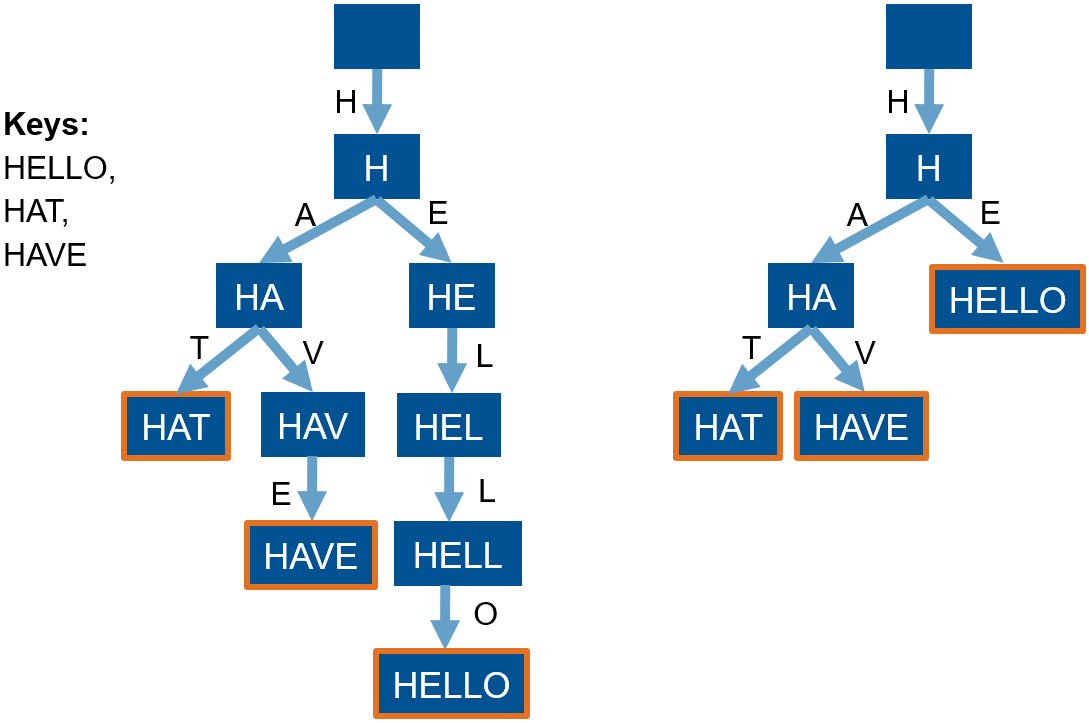
\includegraphics[width=0.5\textwidth]{images/01-trie-radix-tree-example.PNG}
    \caption{A trie with span 8 (1 byte per character) storing the keys "HELLO", "HAT", and "HAVE" on the left and its radix tree variant on the right. Nodes marking the end of a word are outlined.}
    \label{fig:trie}
\end{figure}

Tries have the following interesting properties:
\begin{itemize}
    \item Tree height and complexity do not depend on the number of keys stored $n$ but rather
    the key length $k$. As we will see later in Section 4, this means that its performance is mainly impacted not by
    the amount of keys present as in other search trees but by the skewness of those keys.
    \item Tries require no rebalancing.
    \item All insertion orders result in the same tree.
    \item Keys are stored in lexicographic order.
    \item Keys are stored implicitly along paths. (This is not directly true for radix trees and can differ with implementations.)
\end{itemize}

The span of a trie is the number of bits making one partial key. The fanout of a node is the number of children 
a node can have maximum. The simplest implementation for a trie of span $s$ is to have a fanout of $2^s$ on 
each node. This means that when storing the children in a pointer array of size $2^s$, the partial key can be used 
directly as index into this array to find the next child without having to make any comparisons.
With this, the height of a given trie storing keys of $k$ bits is bound by $\lceil k/s\rceil$, and increasing 
the span results in a lower trie height which is desirable as the height dictates the time complexity for almost 
all operations.

On the other hand, increasing the span results in an exponentially higher fanout, thus requiring more space as even 
if few children exist, the array will be filled with null pointers wasting memory. 
For this reason, having a very high span is generally impractical. The Generalized Prefix Tree (GPT) \cite{mci/Boehm2011} 
has a span of 4, and the radix tree implementation used in the Linux kernel (LRT) uses 6 bits \cite{corbet2006lrt}. 
The Adaptive Radix Tree (ART) \cite{6544812}, as depicted in Figure \ref{fig:trie-mem}, while using a span of 8, manages to have both 
fairly low memory consumption as well as a small tree height.

\begin{figure}
    \centering
    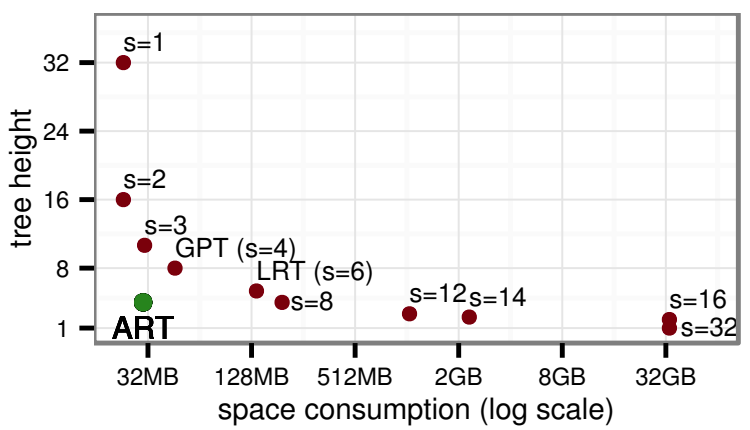
\includegraphics[width=0.4\textwidth]{images/02-trie-memory-consumption.png}
    \caption{Comparison of tree height versus space consumption for different radix tree spans $s$ when storing 1M uniformly distributed 32 bit integers with 8 byte pointers.
    Source: \cite{6544812}}
    \label{fig:trie-mem}
\end{figure}

The key idea in lowering memory consumption while maintaining a high span for tries is to adaptively use nodes 
with different fanouts based on the number of actual children present. One of the first data structures to utilize such 
adaptive nodes was the Judy Array \cite{baskins2004judy} which was invented by Doug Baskins and developed at 
Hewlett-Packard research labs as a general associative array. However, due to its patent and overall complexity, 
it has not yet been researched as much. Also, its original, almost two-decade-old design has flaws like assuming 
16 byte cache-line sizes and not utilizing SIMD.

The rest of this paper is organized as follows. We first introduce the Adaptive Radix Tree as an index structure 
and explain its key design features. In Section 3, we show how to convert different key types to binary-comparable keys to 
index in ART. Section 4 evaluates ART by comparing its performance and memory consumption first in 
microbenchmarks and then the TPC-C benchmark. Section 5 discusses related work and research done since the 
original proposal of ART back in 2013. The final part draws a conclusion and discusses future work.

\section{The Adaptive Radix Tree}

The Adaptive Radix Tree (ART) was first proposed by Leis et al. \cite{6544812} as a performant, order-preserving 
in-memory index structure. Being an adaptive radix tree similar to Judy Arrays it uses multiple node types 
with different fanouts to drastically lower memory consumption and vertical compression to reduce the overall tree 
height and further memory usage while improving performance.

\subsection{Horizontal Compression (Adaptive Nodes)}
ART uses four different node types, each with a different fanout but the same span 
of 8, to adaptively change between them based on the actual number of child nodes. This way, less space is wasted 
storing null pointers. Additionally, storing the children in sorted order allows for range scans along nodes. The node types 
illustrated in Figure \ref{fig:nodes} are named after the maximum number of children 
they can store. For better cache line utilization during searches ART stores partial keys and child pointers in two 
seperate arrays as opposed to storing key-pointer pairs in one single array:

\begin{figure}
    \centering
    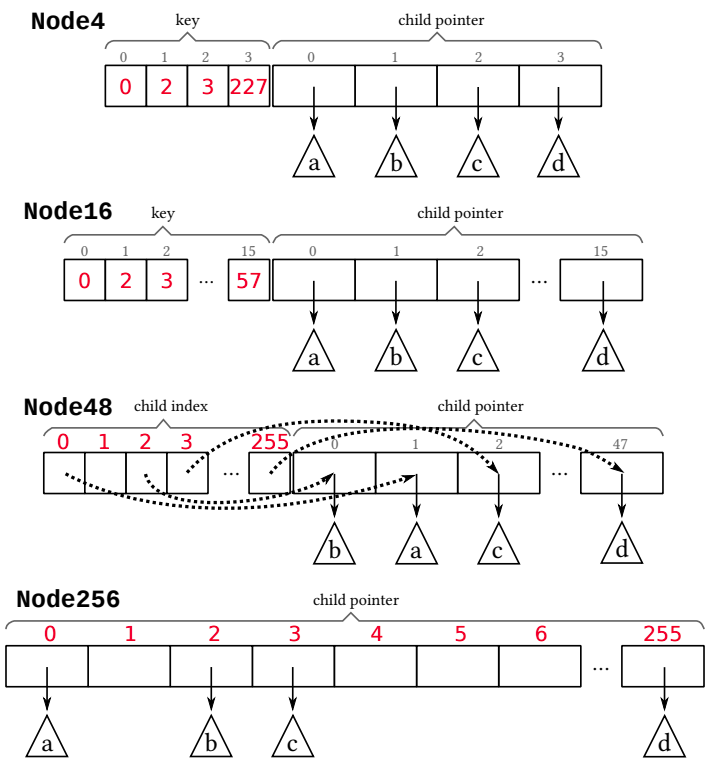
\includegraphics[width=0.5\textwidth]{images/03-art-node-types.png}
    \caption{Different node structures used by ART. For each node, the partial keys 0, 2, 3, and 255 are mapped to the subtrees a, b, c, and d, respectively.
    Source: \cite{6544812}}
    \label{fig:trie-mem}
\end{figure}

\textbf{Node4:} Stores up to 4 children by maintaining a sorted array with size 4 of partial keys where the searched index 
in the key array is also the index into the child array for the associated child.

\textbf{Node16:} This node stores up to 16 children in the same way as Node4. Searching for a key can be done 
efficiently using SIMD instructions.

\textbf{Node48:} As the number of partial keys to differentiate increases, searches become more expensive, even in 
sorted order. Therefore Node48 uses a full 256-sized byte array to hold all possible partial keys. However, as this 
node only stores up to 48 children, our child array is only of size 48. ART thus stores the index into the 
child array as value in the key array, which is indexed directly using the partial key.

\textbf{Node256:} Finally, the largest node stores children in the classical trie approach with a child 
array of size 256 so that, similarly to Node48, the partial key is used directly as index.

Additionally, all nodes have a header of constant size storing the node type, the number of non-null children, 
and a prefix variable containing information about the compressed path (see Section 2.2).

\subsection{Vertical Compression}
As a radix tree, ART implements two techniques often used in tree-like structures: lazy expansion and path compression. 
With these ART compresses node chains where each node only has a single child, further reducing tree height and space 
consumption while improving performance.

\textbf{Lazy Expansion:} 
Lazy expansion refers to the standard radix tree approach introduced by Morrison \cite{10.1145/321479.321481} to 
expand nodes lazily upon insertion. New nodes are therefore only created as long as they are needed to distinguish between at least two different keys. This can be seen
again in Figure \ref{fig:art-vertical-compression} where the key "FOO" is lazy expanded, meaning the path for storing the
two "O"s is omitted. Since paths to leaves may be compressed, this requires the full key to be stored alongside its value 
or be retrievable based on the value. The latter is most often the case in database indexes, where the value 
is used as a reference to a data tuple also containing the key.

\begin{figure}
    \centering
    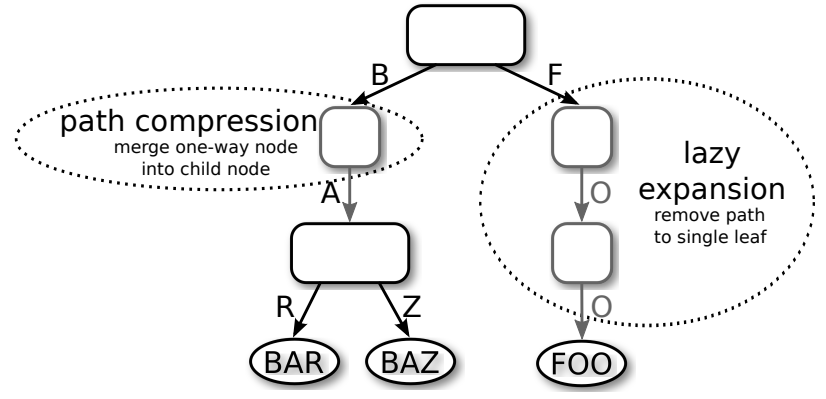
\includegraphics[width=0.45\textwidth]{images/04-art-vertical-compression.PNG}
    \caption{Lazy expansion and path compression in effect.
    Source: \cite{6544812}}
    \label{fig:art-vertical-compression}
\end{figure}

\textbf{Path Compression:}
Similarly, path compression removes nodes containing only one child and gets applied during insertion when expanding 
upon a previously lazy expanded key or deletion. Figure \ref{fig:art-vertical-compression} shows an example where 
the node for key part "A" would be omitted. To still be able to compare the full key Leis et al. identify three different approaches:
\begin{itemize}
    \item Pessimistic: Each node can store a variable length part of the key in its header. 
    Upon compression, the compressed key part is stored in the parent. When traversing a node, the additional
    stored key part is compared first, and then, in case of a match, we continue with the next partial key.
    \item Optimistic: Instead of storing the omitted key part itself, the parent node only stores the number of 
    omitted nodes. Thus, traversing a node just skips this number of partial keys. When reaching a value, we will 
    again have to compare the entire key to ensure the optimistically skipped key part matches.
    \item Hybrid: While the pessimistic approach does not require rechecking keys, it needs to store a variable length 
    key part in its header leading to further cache misses when skipping long key parts. This differs from the 
    optimistic approach, where each node only stores a single number.
\end{itemize}

ART uses the hybrid approach and stores the key part pessimistically for up to 8 bytes. If more than eight nodes 
get compressed, it switches to the optimistic approach.

\subsection{Storing Values}
Values associated with keys can be stored in different ways:
\begin{itemize}
    \item Single-value leaves: The classical approach of storing a value in an extra leaf type node.
    \item Multi-value leaves: Multiple leaf node types based on the inner node types (Section 2.1) 
    but storing values instead of child pointers.
    \item Combined pointer/value slots: When values fit the size of a pointer storing the value at the place instead 
    of a child pointer can be done via pointer tagging or using an additional bit per pointer.
\end{itemize}

Single-value leaves increase the tree height but can differentiate keys of different lengths as opposed to 
multi-value leaves. Combined pointer/value slots is generally the best approach. On typical 64 bit architectures, 
the lowest bit of an alleged pointer can be set to indicate an actual stored value of up to 63 bits length as 
pointers are 8 byte aligned.

\subsection{Algorithms \& Space Consumption}
The original ART paper \cite{6544812} also shows and explains pseudo code for the search, insert, 
bulk loading and delete which is ommitted here for brevity.

Similarly, Leis et al. also presented a proof for the worst-case space consumption per key, which is bounded by 52 bits even for
arbitrarily long keys. As we will see in Section 4, this space consumption per key can be in practice as low as 8.1 bits
for dense keys.

\section{Constructing Binary-Comparable Keys}

\begin{figure*}
    \centering
    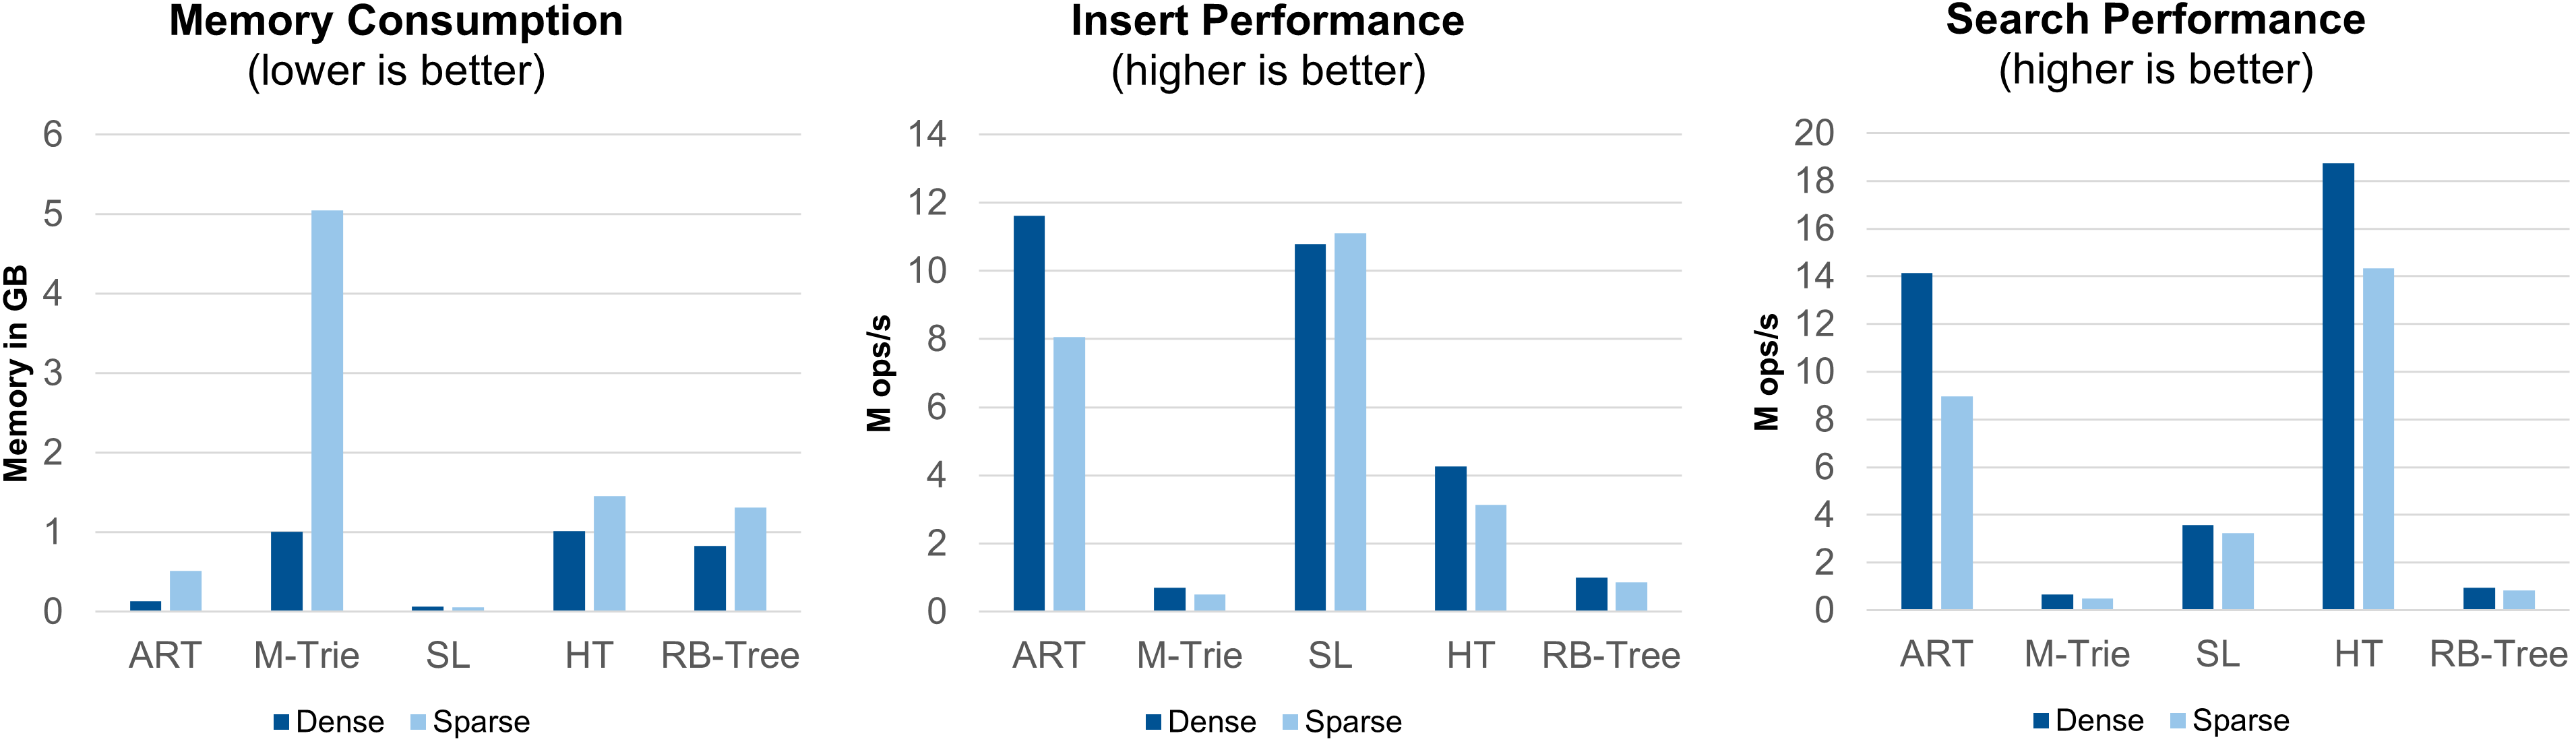
\includegraphics[width=\textwidth]{images/06-art-micro-benchmark-16.PNG}
    \caption{Benchmark results for 16 million 32 bit unsigned integers.}
    \label{fig:art-micro-benchmark-16}
\end{figure*}

To preserve order on keys in a radix tree and therefore allow range-based queries, it is required that the bitwise representation of a key is 
ordered in the same way as the key in its own context. This is the case for some key types like ASCII encoded strings 
as the binary representation of 'A' is smaller than the one of 'B' and so forth. However, for general types, this may not be the case.

For this reason, Leis et al. proposed various key transformations for common types such that the binary 
representation of a type implies the same order as the type itself.

Having the same order means for two values $a$, $b$ of the same type
\[a < b \iff bin(a) <bin(b)\qquad\text{(same for $>$ and $=$)}\]
where $bin(x)$ is the binary representation of $x$.

The transformation for the most common types are as follows:
\begin{itemize}
    \item Unsigned Integers: The binary representation of unsigned integers is already ordered correctly. 
    However, when operating on keys in memory, the endianness generally matters as for little endian, the bytes 
    have to be swapped first. This can also be done implicitly in the implementation.
    \item Signed Integers: For signed two-complement integers, the sign bit must first be flipped. Then it can be 
    stored like an unsigned integer.
    \item Strings: The Unicode Collation Algorithm (UCA) already defines transformations for strings to 
    binary-comparable keys.
    \item Compound Keys: Keys with multiple types can be transformed by transforming each type individually and 
    concatenating the result.
\end{itemize}

Additionally the authors of ART also showed transformations for floats and nullable types \cite{6544812}.

\section{Evaluation}

In this section, we evaluate ART first with our implementation and with microbenchmarks comparing the
results to the same microbenchmarks used in the original ART paper. Then we show Leis et al. results and evaluation 
for performing the
standard OLTP benchmark TPC-C.

Our ART implementation \cite{fritschart} uses combined value/pointer slots on 64 bit architecture with SIMD instructions for Node16 
and does not include path compression, only storing a 2 byte header (node type and number of non-null children).
Leaving out path compression does not result in any performance loss due to the keys of the microbenchmarks
being only 32 bits long. At such short lengths, path compression generally introduces more overhead and 
additional memory consumption, so it is better to deactivate it.

Our benchmarks were run on an Intel Core i5-8400 CPU with around 3.7 GHz reported clock rate during benchmarks.
It has 6 cores, 6 threads, 8 MB shared, last-level cache. Our system has 16 GB dual-channel DDR4-2666 RAM. As operation system, we used Windows 10.0.19044 and the MSVC v143 compiler with flags /O2 and /Ob3.

\subsection{Micobenchmarks}

The microbenchmarks uses 16 million 32 bit unsigned integers as keys without another associated value. We compare ARTs 
performance to a Trie implementation storing child pointers or the last partial key in a std::map (M-Trie), a 
Sorted List (SL), a chained hash-table (HT) using the std::unordered\_set implementation, and a red-black tree 
(RB-Tree) using the std::set implementation.

We split our datasets into dense and sparse keys, where sparse are uniformly random 32 bit keys and dense keys only
range from $0$ to $n-1$ where $n$ is the number of keys inserted (16 million).

While the dense 16 million key set effectively only uses 24 bit keys ($\log_216000000\approx24$)
the sparse set always uses full random 32 bit keys.

For both benchmark sizes and each dataset, we measured memory consumption in GB, insert, and positive/successful search performance with million operations per second. 
The results can be seen in Figure \ref{fig:art-micro-benchmark-16}.

\textbf{Memory Consumption:} We see that ART uses less memory than the other data structures except for the Sorted List, which stores all keys in a single vector and thus has almost optimal memory consumption. Additionally, for the 
trie-based structures, the difference in memory between dense and sparse is due to the nature of common prefix
compression of tries. Compared to the M-Trie, ART does not have such a huge increase in memory consumption for the sparse set
because of its vertical compression (specifically lazy expansion in this case).

\textbf{Insert Performance:} ART outperforms all other data structures except the Sorted List. 
Note that for the Sorted List, insertion is done as bulk insert $O(n\log n)$ rather than constantly 
inserting a new key at the correct position shifting all later keys $O(n^2)$. Otherwise, its performance would be significantly
worse. Bulk insertion for ART also improves performance but mostly for dense sets \cite{6544812} with a factor of 2.5.

\textbf{Search Performance:} For single-point searches, ART is only outperformed by the Hash-Table, which has amortized
constant lookup time. The Sorted List with binary search performs the third best.

Overall these benchmark results are comparable to the results in the original ART paper \cite{6544812}. 
The only significant difference is that in Leis et al. search benchmarks, ART consistently performed best for the 
dense set, even topping the hash table. This can be explained by the fact that the hash function chosen by the authors 
MurmurHash64A \cite{murmur} while considered very robust is slower than a simpler hash function.

Because of their results, Leis et al. concluded that only a hash table could be competitive in terms
of performance. However, we will see in Section 5 that state-of-the-art hash tables can have lower memory consumption
or outperform ART's search performance by several factors.

\subsection{End-to-End Evaluation}

\begin{figure}
    \centering
    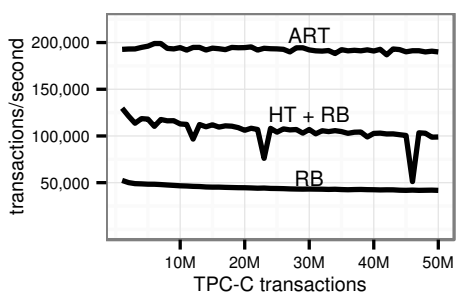
\includegraphics[width=0.4\textwidth]{images/07-art-tpc-c.png}
    \caption{TPC-C performance.
    Source: \cite{6544812}}
    \label{fig:art-tpc-c}
\end{figure}

As the final evaluation, ART was implemented in the main-memory database system HyPer \cite{5767867} and evaluated 
using the TPC-C benchmark \cite{6544812}. Its performance was compared by using a red-black tree index and a 
combination of a red-black tree and a hash table index. The results are shown in Figure \ref{fig:art-tpc-c}. ART 
performs twice as fast as the combination of hash table and red-black tree, where the performance dips of the combination of indexes can be 
explained by the hash table reaching its load balance and doing a complete re-hash.

Further results of this benchmark were ART only using half as much space as the hash table and the red-black tree. 
In practice, ART used around 8.1 bits per key for dense sets and up to 32.6 bits per key for sparser sets which 
again matches the results of our microbenchmarks in Section 4.1.

It also shows that both vertical compression techniques significantly impact overall tree height, 
reducing it from as much as 40 down to 8.1 on average.

\section{Related Work}
As the authors of the original ART paper concluded that only a hash table was competitive with the performance of ART \cite{6544812} 
with ART still outperforming it in some cases, Alvarez et al. published a paper \cite{7113370} in response further comparing ART to
not only a variety of different hashing schemes and hash functions but also the Judy Array, another adaptive radix tree.

In it, they showed that with better hashing schemes such as Cuckoo-Hashing \cite{PAGH2004122} instead of a chained hash table
and simpler hash functions such as multiplicative hashing instead of Marmur hash tables do outperform ART by several factors in
both insertion and single-lookup performance or other hash tables achieve similar performance but only require half the space.

Compared to Judy Arrays, ART achieved double the performance while also needing around twice as much space.

Another more recent paper by Wang et al. compared ART to more state-of-the-art order-preserving index structures such 
as the Bw-Tree, MassTree, and a B\textsuperscript{+}-Tree version optimized for main memory usage. They also ran multi-threaded
benchmarks using a synchronized version of ART presented by Leis et al. \cite{10.1145/2933349.2933352}. Their results show
that ART generally performs better or similar than all other indexes in both performance and memory consumption except for
range-based queries where the B\textsuperscript{+}-Tree outperforms all other indexes because of its spacial locality of 
leaf nodes.

In recent years further variants of ART have been developed like HOT \cite{10.1145/3183713.3196896}, where nodes can have different spans to improve performance
on sparse sets, or START \cite{9094133} where lower level nodes are dynamically combined and optimized using
a cost model and optimizer, further improving performance and memory consumption.

\section{Conclusion and Future Work}

Concluding ART is a synchronized, general purpose, order-preserving index structure that is space efficient, 
generally outperforms other order-preserving indexes in performance.
It is, however, outperformed by state-of-the-art hashing-based indexes in at least single-threaded environments.

The Adaptive Radix Tree is used as an index in main memory database systems like HyPer \cite{5767867} or DuckDB \cite{10.1145/3299869.3320212}.

With the Judy Array patent just expired, it remains to be seen how ART would compare to a modernized version of
Judy Arrays and if ART could even benefit from some of Judy Arrays' design choices like Judy Pointers, to reach 
Judy Arrays' memory efficiency.

\bibliographystyle{ACM-Reference-Format.bst}
\bibliography{refs}

\end{document}
\endinput